\documentclass{beamer}

\usepackage{times}
\usepackage[orientation=portrait,size=a0,scale=1.4]{beamerposter}
\usetheme{JuelichPoster}

%\setbeamertemplate{title banner}{Mitglied der Helmholtz-Gemeinschaft}
\setbeamertemplate{logo partner2}[show][0.55]{figures/logos/grs_logo.pdf}
\setbeamertemplate{logo partner1}[show][0.55]{figures/logos/rwth_logo.pdf}
\setbeamertemplate{author}[show][0.8]{figures/oliver_schillinger.jpg} %Here is where your photo is suppose to go
\setbeamertemplate{itemize items}[square]
\setbeamertemplate{enumerate items}[default]

\newcommand{\shift}{\vspace*{-4cm}}
\newcommand{\shiftmore}{\shift \vspace{-2cm}}

\begin{document}
\begin{frame}[t]

  \shift  \shiftmore

  \frametitle{  \shiftmore \Large Structure of Lipase-CitAP Fusion Protein}
  \framesubtitle{   \shiftmore  Oliver Schillinger (PhD student)}
  
  \begin{columns}[T,onlytextwidth]
    \begin{column}[T]{.48\linewidth}
      \vbox to .88\textheight{

% ============================================================================ %

        \begin{block}{Motivation}

            \begin{columns}[t]
                \column{.44\textwidth}
                \begin{itemize}
                    \item \textit{Bacillus subtilis} Lipase A
                    \item Citrate receptor CitAP
                    \item Fusion protein: switchable detergent
                    \item \textbf{Known:} Individual structures
                    \item \textbf{Unknown}: Fusion protein structure 
                \end{itemize} 

                \column{.5\textwidth}
                \begin{figure}
                    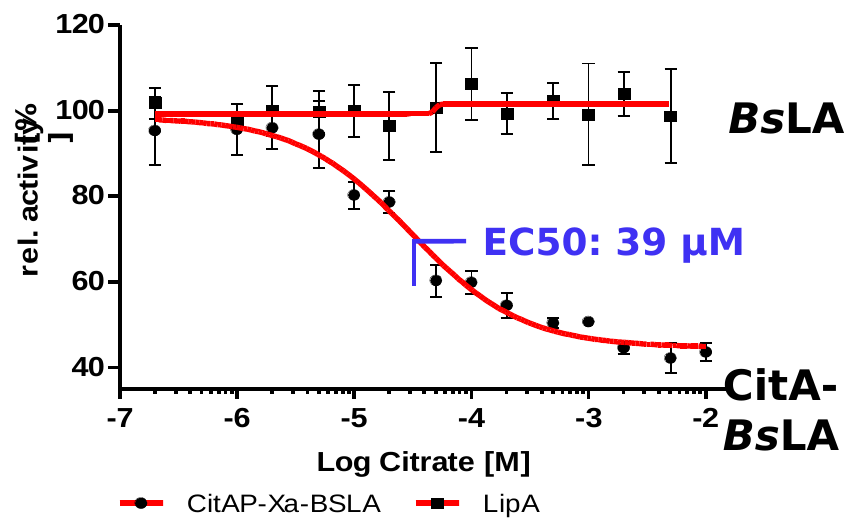
\includegraphics[width=0.9\textwidth]{figures/BSLA_activity/BSLA_activity.png}
                \end{figure}     

            \end{columns}  

        \end{block}

% ============================================================================ %

        \vspace*{1.0ex}

        \vfill 

        \begin{block}{Lipase (BSLA)}

            \begin{center}
            \begin{minipage}{0.8\linewidth}% tweaks the width, makes a new \textwidth
                \begin{itemize}
                    \item Catalyses hydrolysis and synthesis of \textbf{triacylgliycerols}
                    \item Diverse substrate specificity
                    \item Used in industry for
                        \begin{itemize}
                            \item Resolution of racemic mixtures
                            \item Synthesis of esters
                            \item Additive laundry detergent
                        \end{itemize}
                \end{itemize}  
            \end{minipage}
            \end{center}   


            \begin{columns}[t]
                \column{.5\linewidth}
                \begin{figure}
                    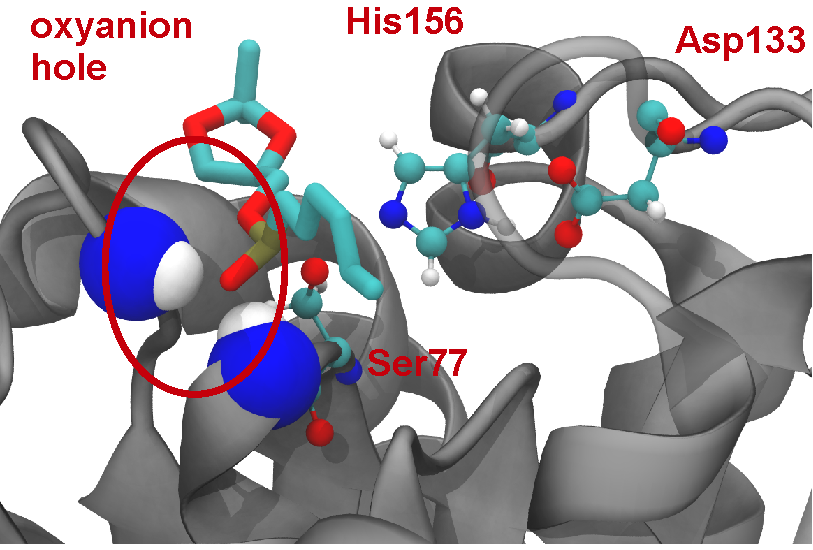
\includegraphics[width=1.0\textwidth]{figures/BSLA_pocket/BSLA_pocket_cartoon.pdf}
                \end{figure}      

                \column{.5\linewidth}
                \begin{figure}
                    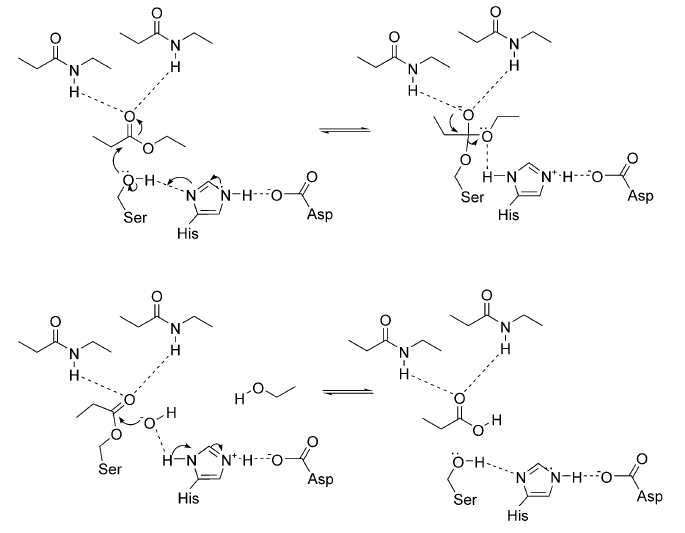
\includegraphics[width=1.0\textwidth]{figures/BSLA_reaction.png}
                \end{figure}     

            \end{columns} 

            \centering
            His156 -- Asp133 distance related to lipase activity 

        \end{block}

% ============================================================================ %

        \vspace*{1.0ex}

        \vfill

        \begin{block}{Citrate Receptor (CitAP)} 

            \begin{columns}[t]
                \column{.55\linewidth}
                \begin{itemize}
                    \item Periplasmic domain of a two component system of a sensor and a response regulator
                    \item \textit{Klebsiella pneumoniae} two component system is essential for the induction of citrate fermentation genes in the presence of citrate
                \end{itemize} 

                \column{.4\linewidth}
                \begin{figure}
                    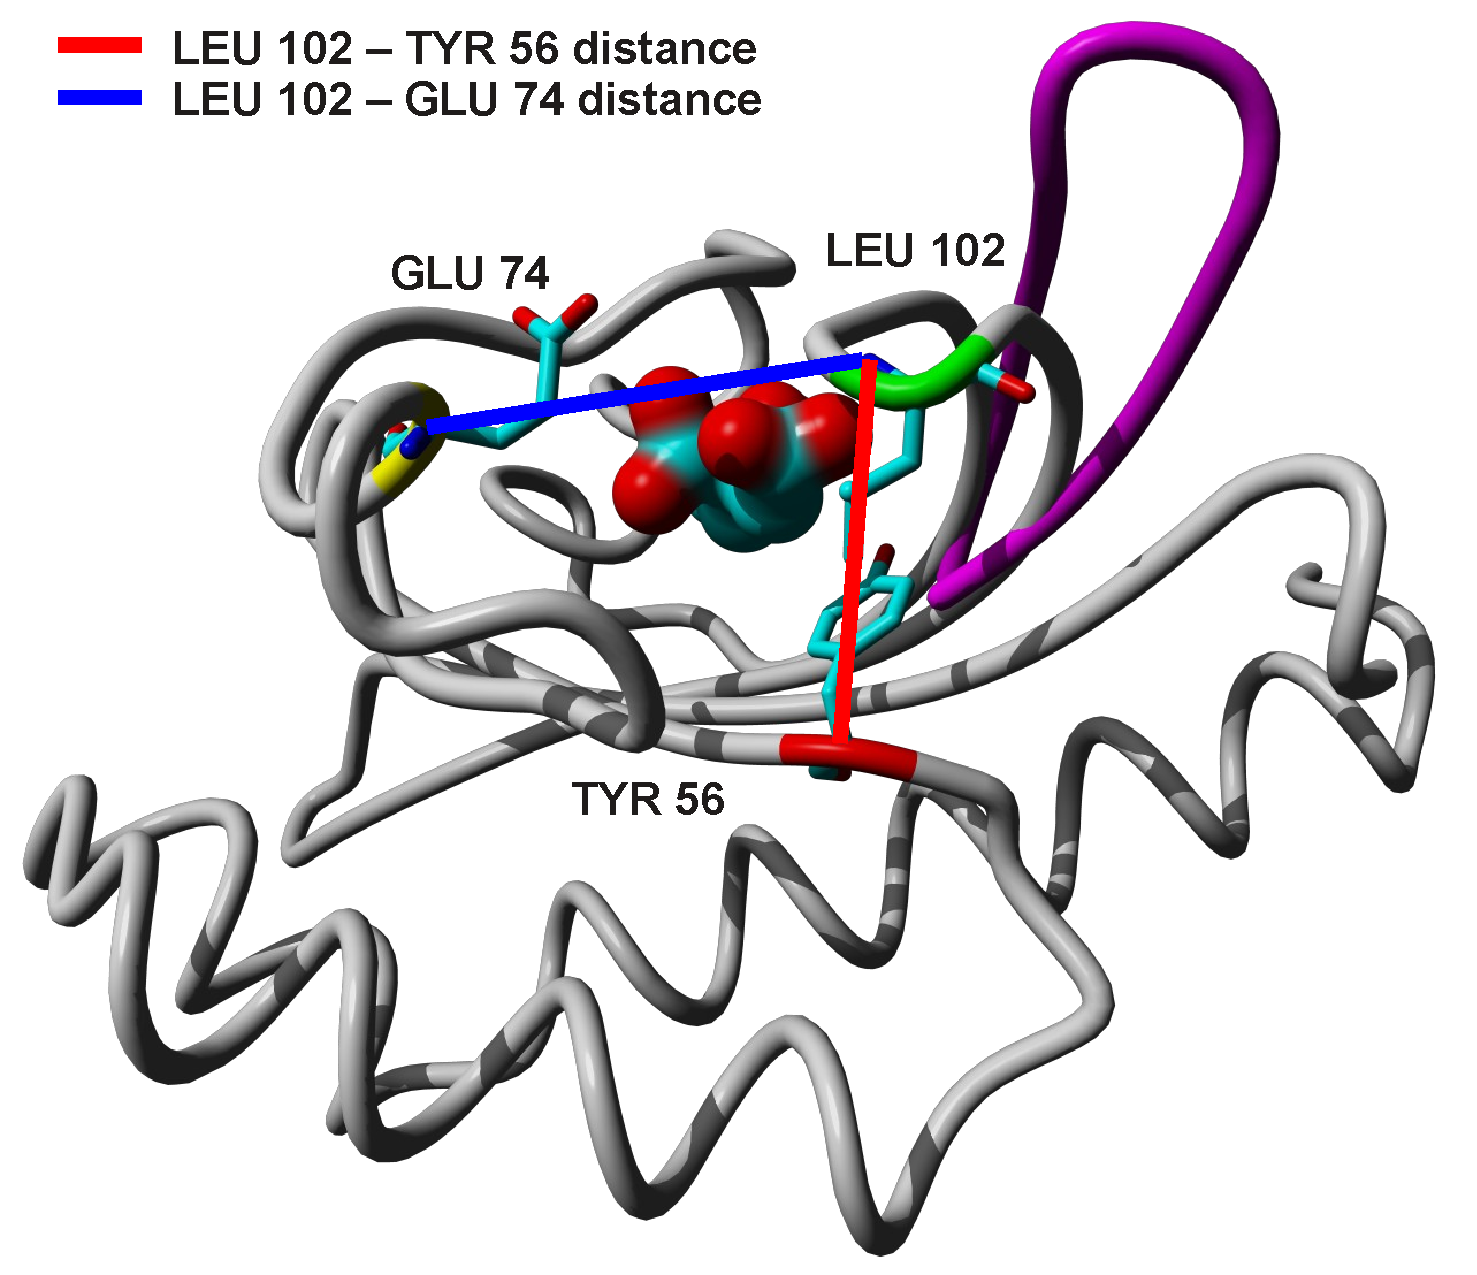
\includegraphics[width=.9\linewidth]{figures/CitA_pocket2.pdf}
                \end{figure}     
                \tiny Bacillus subtilis lipase A with covalently bound Rc-IPG-phosphonate inhibitor (PDB: 1R4Z)

            \end{columns}   

        \end{block}

% ============================================================================ %

        \vspace*{1.0ex}

        \vfill
        \begin{block}{Methods}

            \begin{columns}[t]
                \column{.49\linewidth}
                \begin{figure}
                    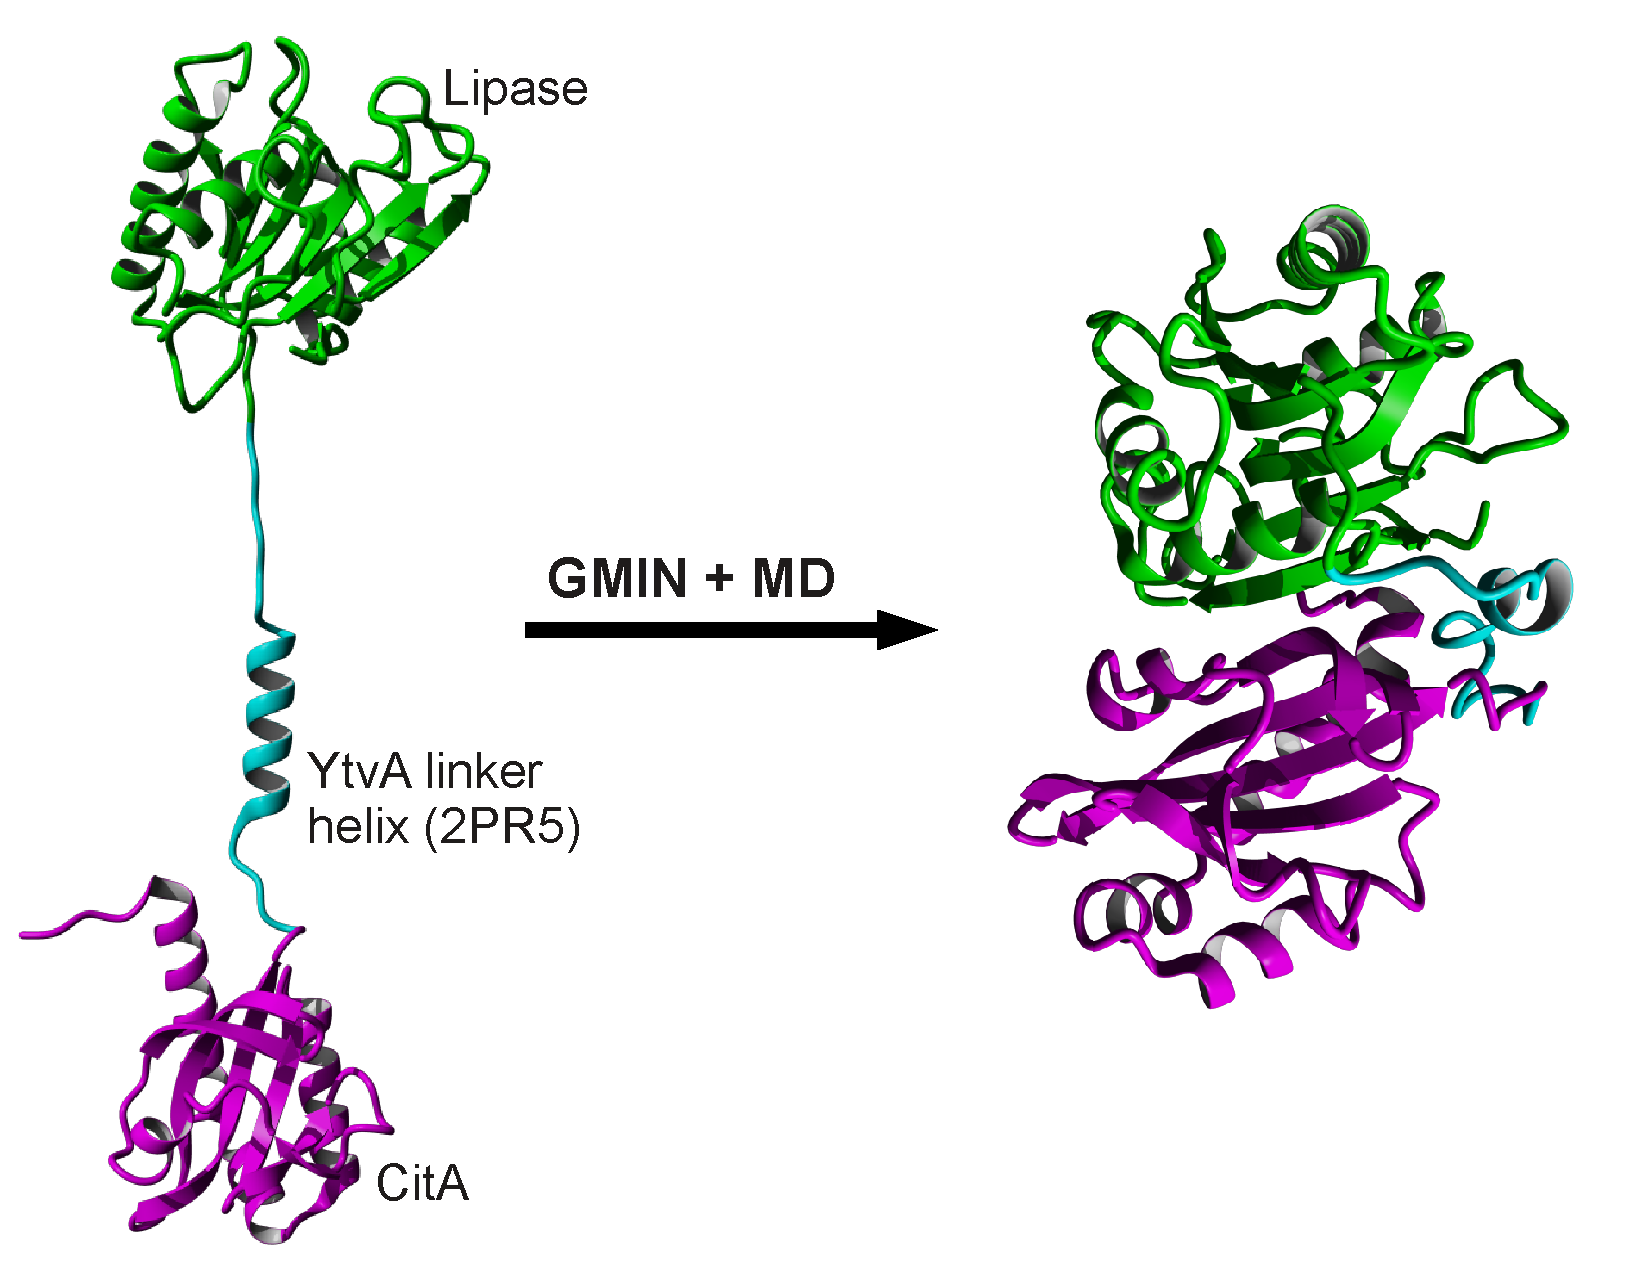
\includegraphics[width=.9\linewidth]{figures/complex/complex_folding.pdf}
                \end{figure}        

                \column{.49\linewidth}
                \begin{figure}
                    Basin Hopping with GMIN
                    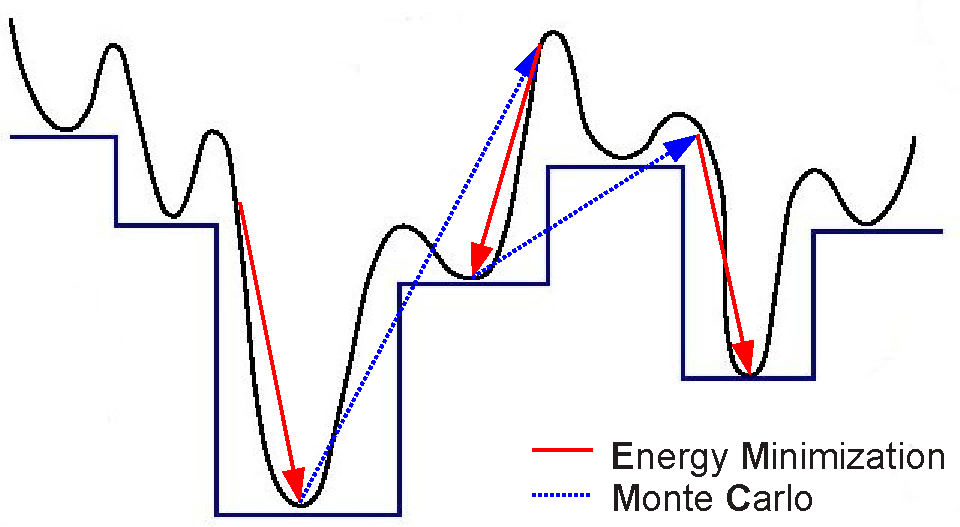
\includegraphics[width=0.9\textwidth]{figures/GMIN/GMIN.pdf}
                \end{figure}         

            \end{columns}    

            \begin{center}
            \begin{minipage}{0.55\linewidth}% tweaks the width, makes a new \textwidth
                \begin{itemize}
                    \item GROMACS
                    \item \textbf{\texttt{amber99sb-ildn-nmr}} force field
                    \item Citrate paremeterization with GAFF
                    \item 10 ns position restrained equilibration
                    \item Gradually decreasing restraining force constant
                    \item 100 ns production runs
                    \item PBC, NPT, PME 
                \end{itemize}  
            \end{minipage}
            \end{center}    

        \end{block}

% ============================================================================ %

%%%%%%%%%%%%%%%%%%%%%%%%%
%       2nd Column      %
%%%%%%%%%%%%%%%%%%%%%%%%%

%    \vfill
    }
    \end{column}
    \begin{column}{.48\linewidth}
        \vbox to .88\textheight{%

% ============================================================================ %

        \vspace*{1.0ex}
  
        \vfill 

        \begin{block}{BSLA Results}
        
            \begin{columns}[t]
                \column{.48\linewidth} 
                \begin{figure}
                    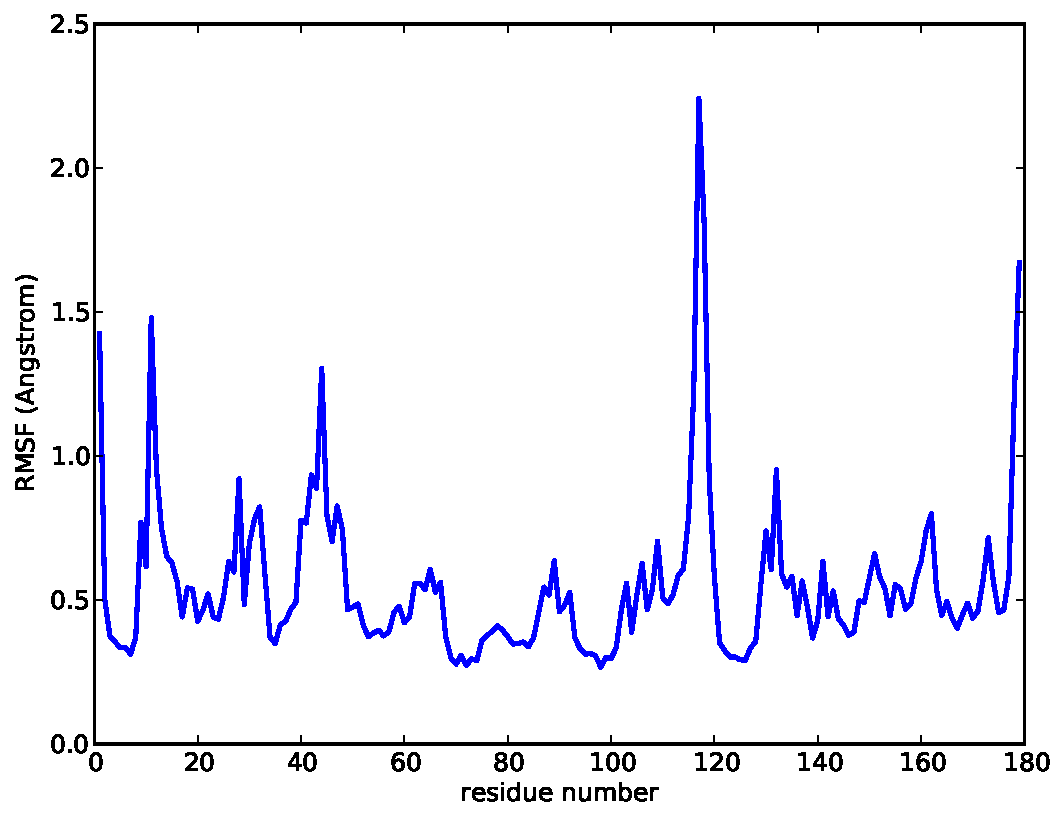
\includegraphics[width=1.0\textwidth]{figures/BSLA_solo/BSLA_solo_rmsf.pdf}  
                \end{figure}       

                \column{.48\linewidth} 
                \begin{figure}
                    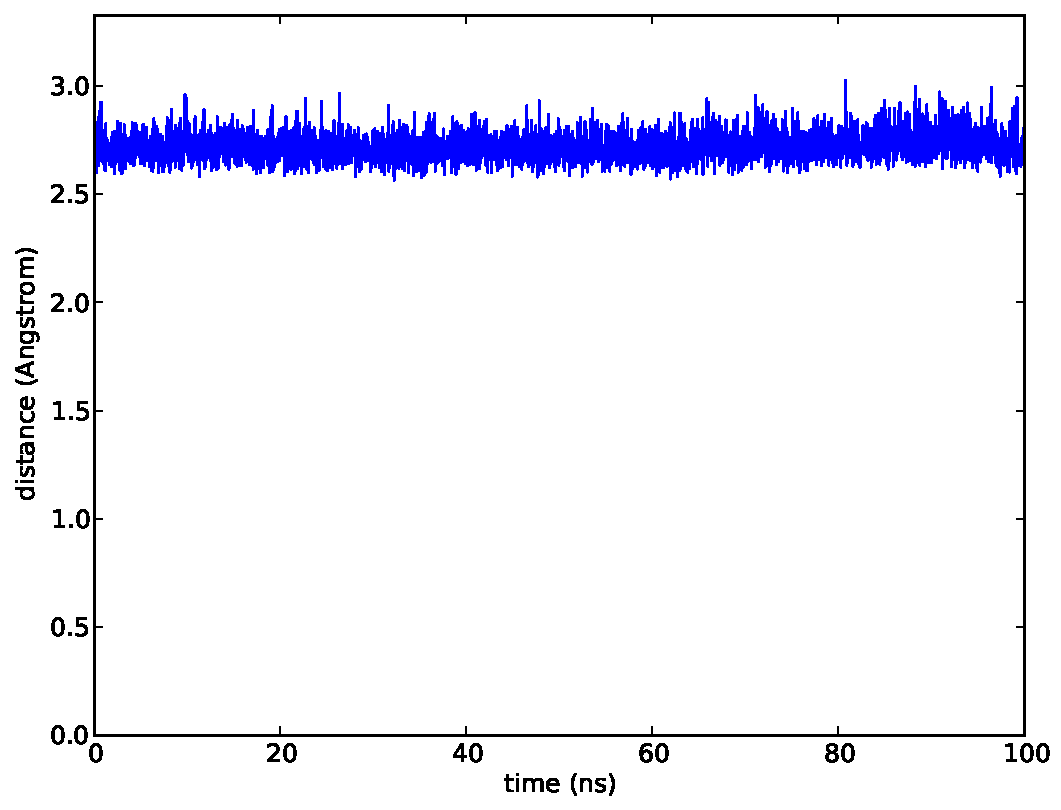
\includegraphics[width=1.0\textwidth]{figures/BSLA_solo/BSLA_solo_dist_ASP133_HIS156.pdf} 
                \end{figure}        

            \end{columns}  

        \end{block} 

% ============================================================================ %

        \begin{block}{CitAP Results}
        
            \begin{columns}[t]
                \column{.48\linewidth} 
                \begin{figure}
                    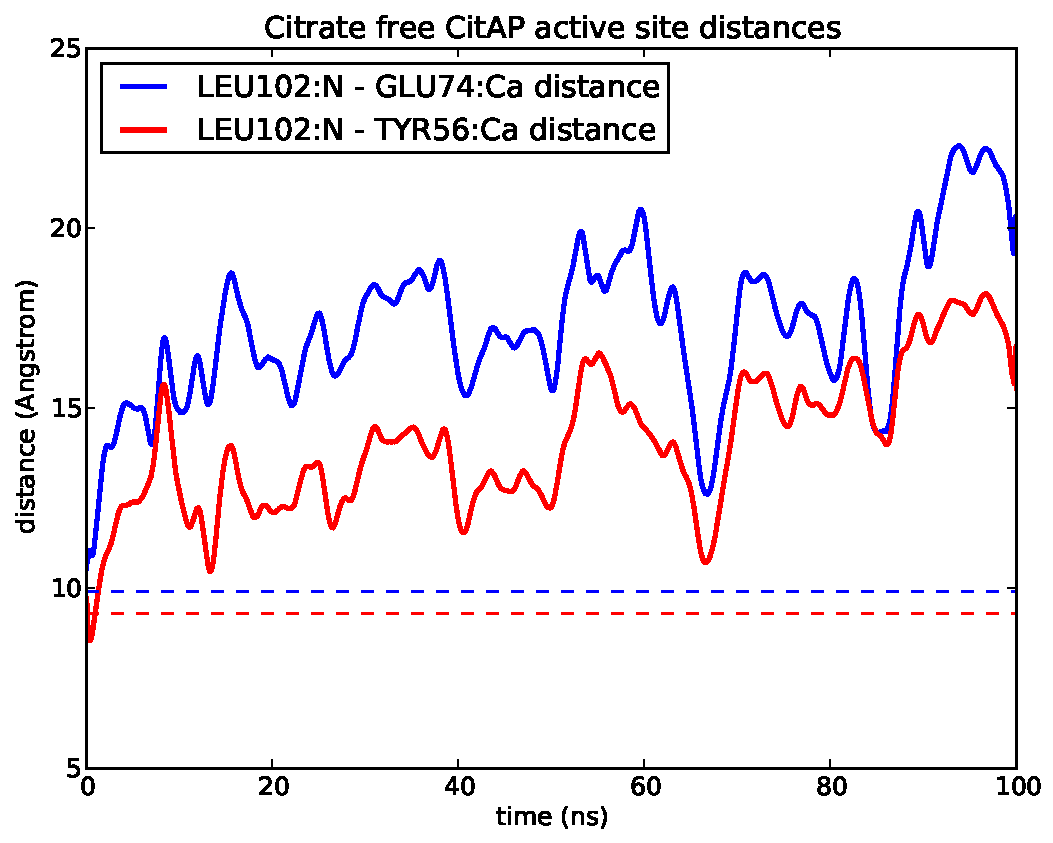
\includegraphics[width=1.0\textwidth]{figures/CitAP_opening/CitAP_dist_free.pdf}
                \end{figure}       

                \column{.48\linewidth} 
                \begin{figure}
                    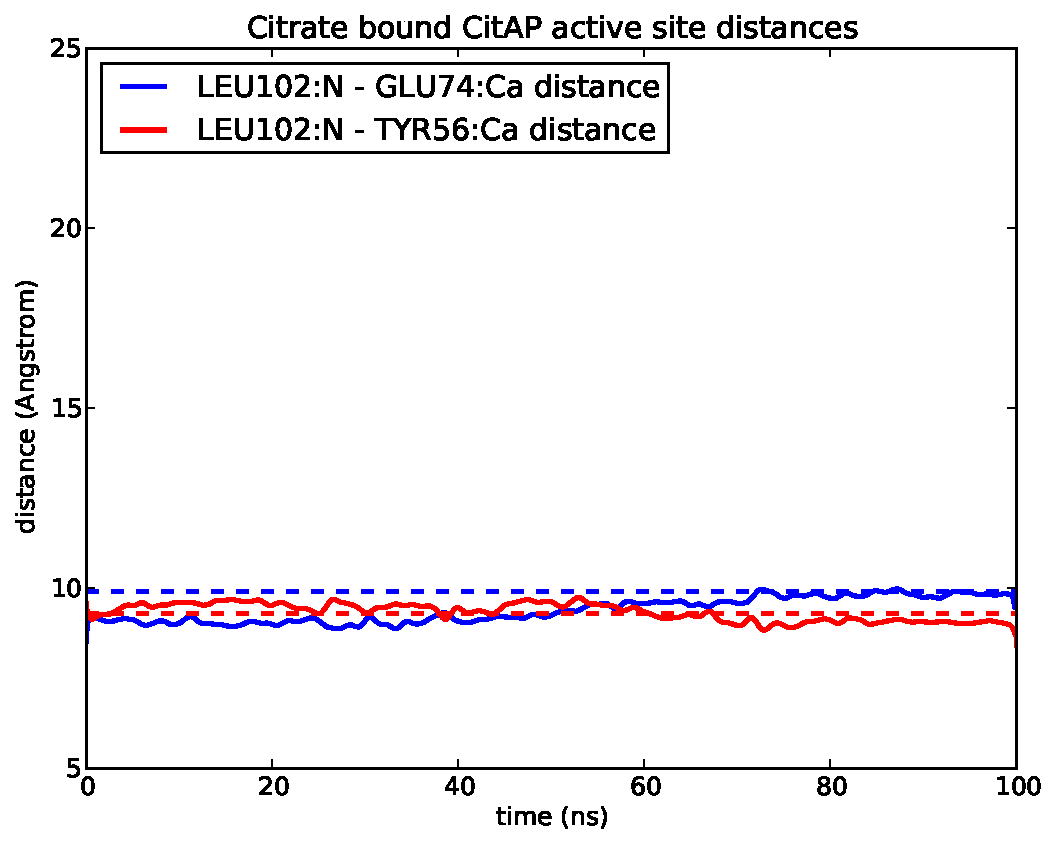
\includegraphics[width=1.0\textwidth]{figures/CitAP_opening/CitAP_dist_bound.pdf}
                \end{figure}        

            \end{columns}  

        \end{block} 
 
% ============================================================================ %

%        \vspace*{1.0ex}
%  
%        \vfill 
%
%        \begin{block}{Basin Hopping Results}
%        
%            \begin{columns}[t]
%                \column{.5\linewidth}
%                \centering
%                Dimensionality Reduction
%                \begin{figure}
%                    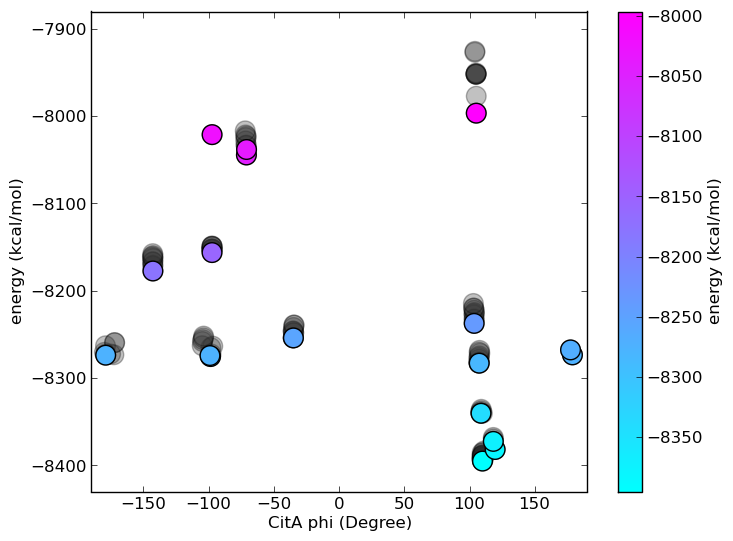
\includegraphics[width=1.0\textwidth]{figures/CitA_phi.png}
%                \end{figure}      
%
%                \column{.5\linewidth}
%                \centering
%                Basin Hopping Structures
%                \begin{figure}
%                    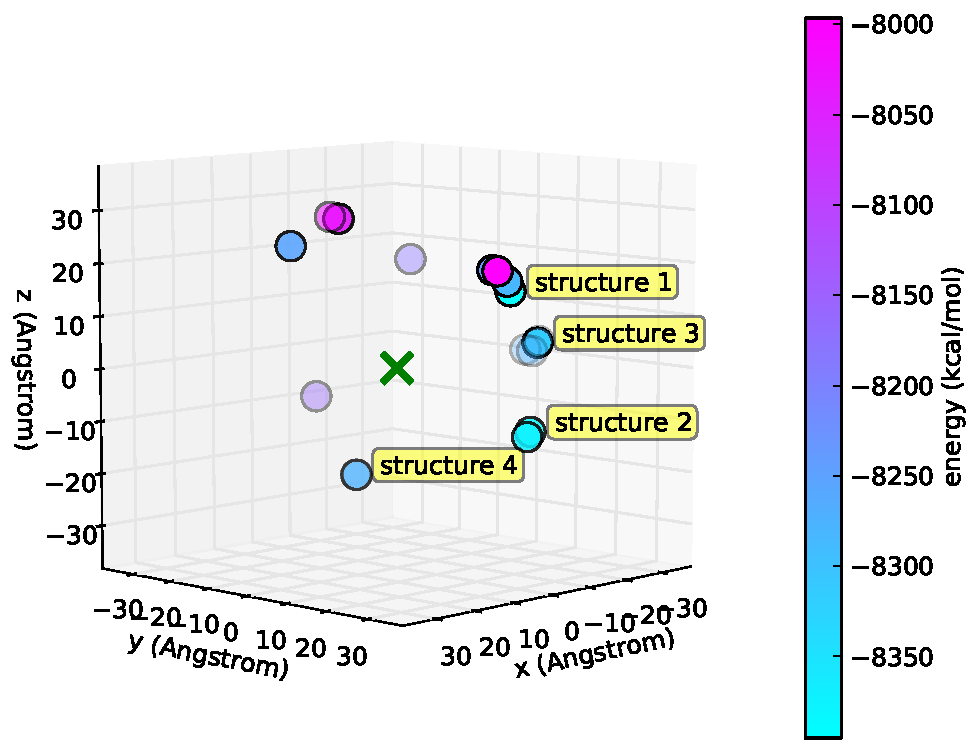
\includegraphics[width=1.0\textwidth]{figures/GMIN/CitA_phi_theta_3D.pdf}
%                \end{figure}     
%
%            \end{columns}   
%
%        \end{block} 

% ============================================================================ %

        \vspace*{1.0ex}
  
        \vfill 

        \begin{block}{Fusion Protein Results}

            \begin{figure}
                \begin{minipage}[]{0.45\linewidth}
                    \centering
                    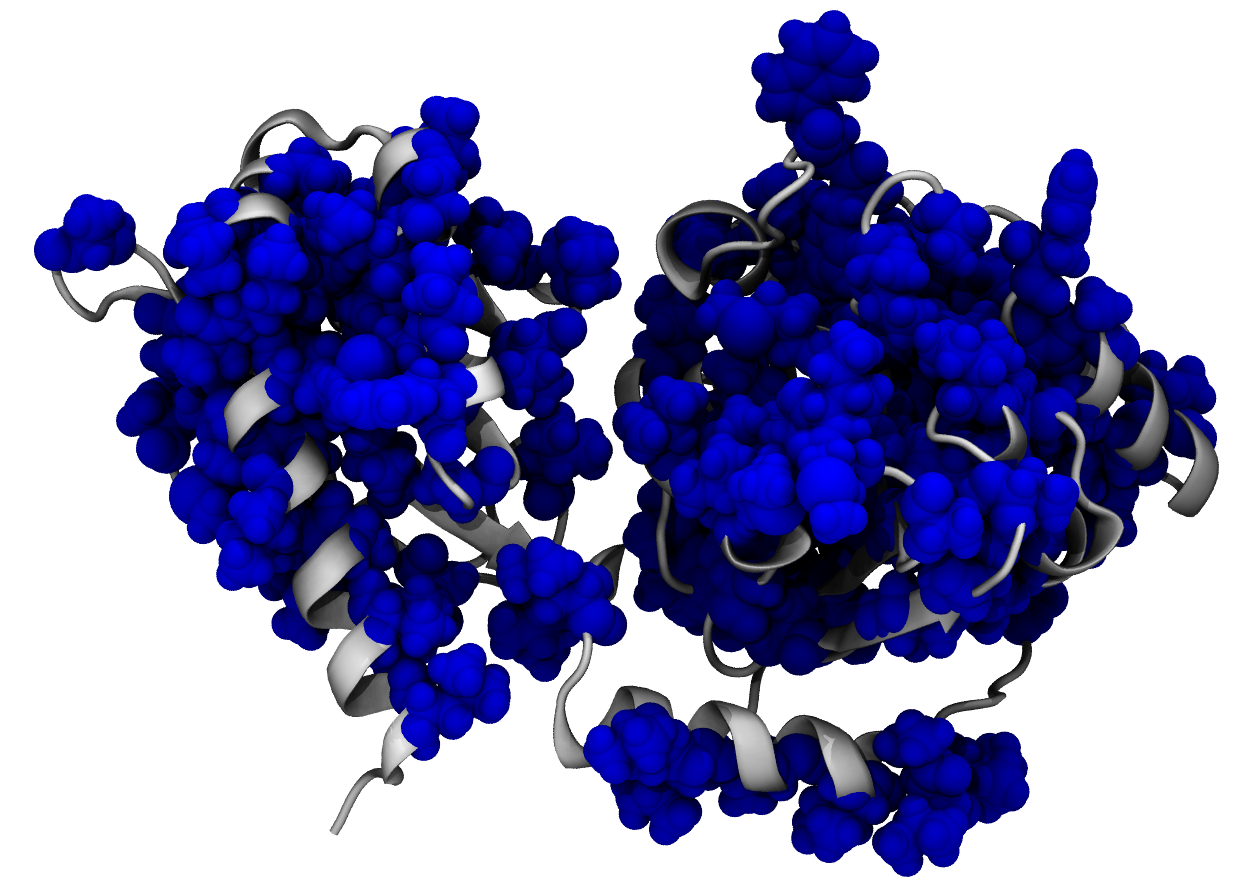
\includegraphics[width=\textwidth]{figures/Complex_hydrophobic_core/hydrophobic_core_linker.png}
                \end{minipage}
            \hspace{0.5cm}
                \begin{minipage}[]{0.45\linewidth}
                    \centering
                    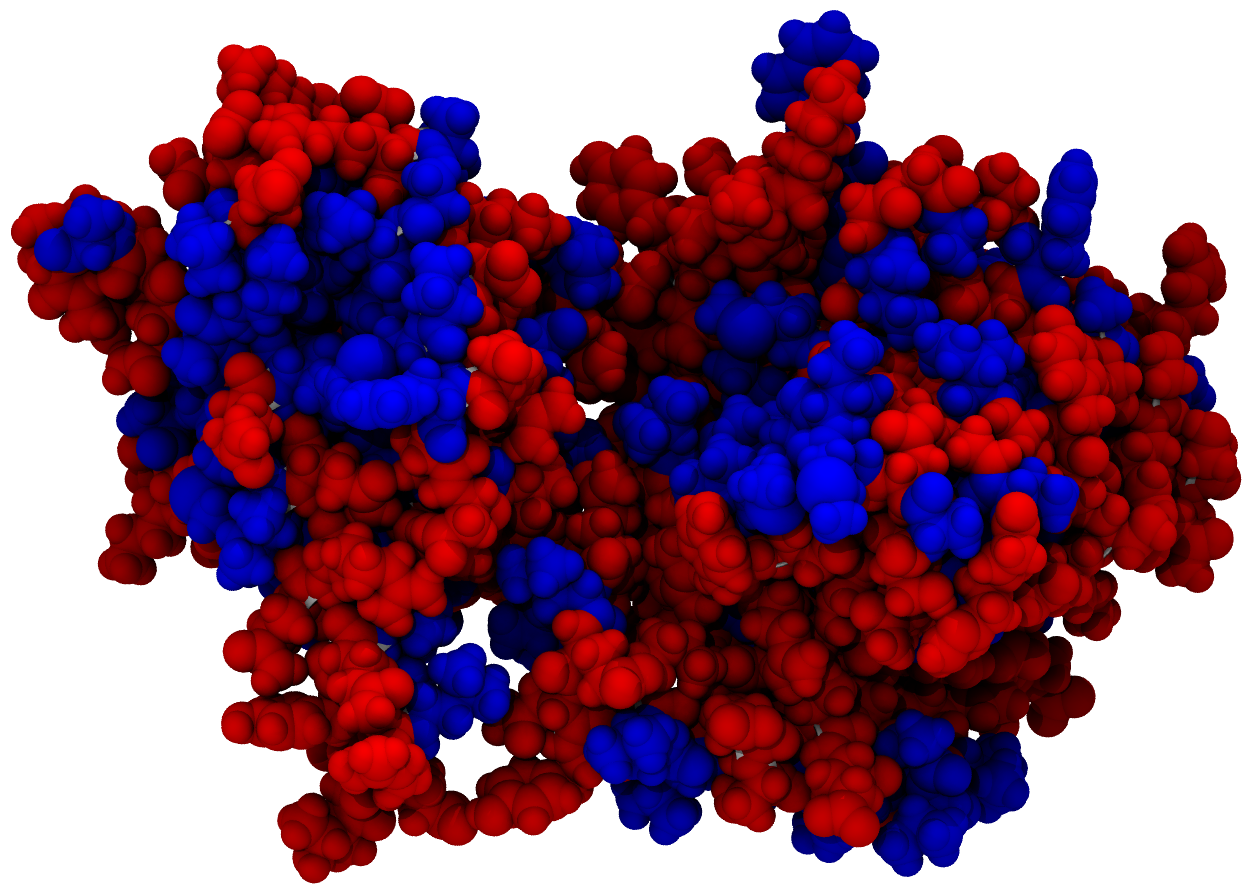
\includegraphics[width=\textwidth]{figures/Complex_hydrophobic_core/protein.png}
                \end{minipage}
            \end{figure}       


            \begin{columns}[t]
                \column{.48\linewidth}
                \begin{figure}
                    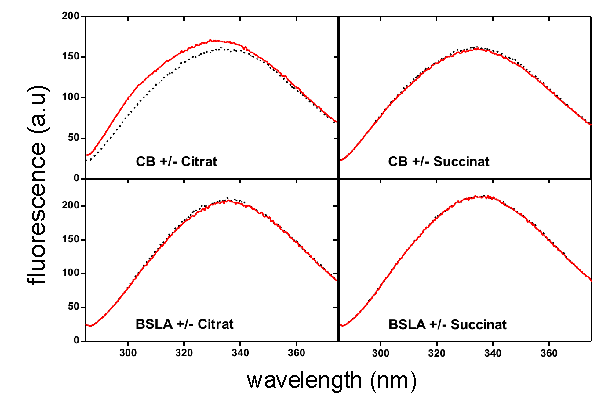
\includegraphics[width=1.0\textwidth]{figures/TyrTrp/TyrTrp_experiment.pdf}
                \end{figure}         

                \column{.48\linewidth}
                \begin{figure}
                    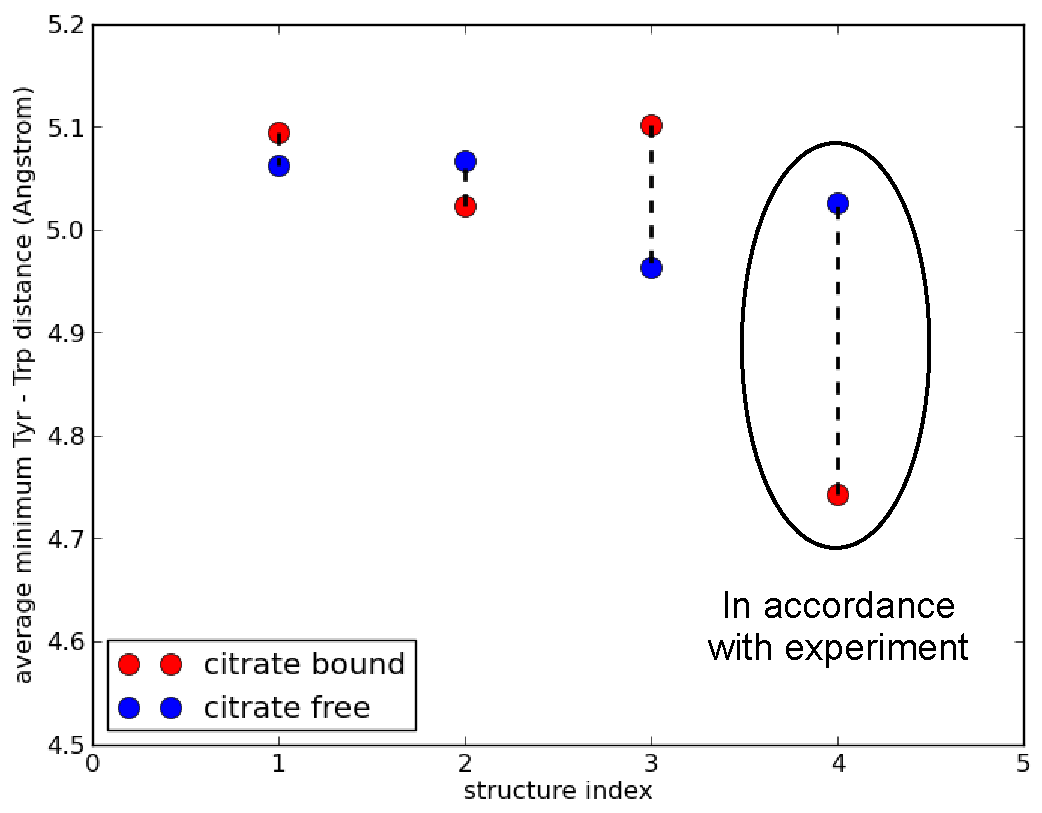
\includegraphics[width=1.0\textwidth]{figures/TyrTrp/average_mindist_TyrTrp_annotated.pdf}
                \end{figure}      

            \end{columns}     

        \end{block}  

% ============================================================================ %

%        \vspace*{1.0ex}
%  
%        \vfill 
%
%        \begin{block}{Fusion Protein MD -- Hydrophobic Contacts}
%        
%
%
%        \end{block}  
 
% ============================================================================ %

        \vspace*{1.0ex}
  
        \vfill 

        \begin{block}{Conclusions}
        
            \begin{itemize}
                \item Solo MD simulations gave expected results
                %\item 4 different fusion protein structures selected
                \item Secondary structure of fusion protein is stable (data not shown)
                \item 2 hydrophobic cores
                \item Systems not equilibrated after 100 ns (data not shown)
                \item Only structure 4 in accordance with TYR/TRP fluorescence
                \item Binding pocket dynamics different in fusion protein (more flexible, data not shown)
                \item No unique active site distance correlation between domains (data not shown)
            \end{itemize} 

        \end{block}  
 
% ============================================================================ %

        \vspace*{1.0ex}
  
        \vfill
  
        \begin{block}{Cooperations}
        Prof. Dr. Karl-Erich Jaeger, Institute of Molecular Enzymtechnology (IMET), FZ J\"uelich
  
      
        \end{block}
   
% ============================================================================ %

   }
    \end{column}
  \end{columns}

  \vspace*{1.5ex}
  \vfill

  \structure{
    \textbf{Contact:} o.schillinger@fz-juelich.de
    \textbf{-}
    \textbf{Website:} http://www.fz-juelich.de/ics/ics-6/DE/strodel
  }
\end{frame}
\end{document}
\endinput   
